\documentclass[conference]{IEEEtran}
\IEEEoverridecommandlockouts

\usepackage[T1]{fontenc}
\usepackage[utf8]{inputenc}
\usepackage{amsmath,amssymb}
\usepackage{booktabs}
\usepackage{graphicx}
\usepackage{tikz}
\usetikzlibrary{arrows.meta, positioning, shapes.geometric}
\usepackage{url}
\usepackage{array}

\title{Market Predictor MLOps Pipeline: Multisource Sentiment, Time-Series Modeling, and Deployment}

\author{\IEEEauthorblockN{Student Name}
\IEEEauthorblockA{Department of Computer Science\\
University Name\\
Email: student@example.com}}

\begin{document}
\maketitle

\begin{abstract}
This project presents an end-to-end market prediction pipeline that ingests live financial and news data, performs sentiment classification, constructs time-series features, trains sequential neural networks, and exposes predictions through a FastAPI service. The system is designed around reproducibility and deployment using DVC, MLflow, Airflow, Docker, and GitHub Actions.
\end{abstract}

\begin{IEEEkeywords}
MLOps, financial forecasting, sentiment analysis, Airflow, DVC, MLflow, FastAPI
\end{IEEEkeywords}

\section{Introduction}
Financial market prediction is a multi-source data problem that benefits from structured ingestion, robust feature engineering, and reproducible model training. This project combines price history from Yahoo Finance with news and social sentiment from Reuters and Reddit to produce a compact pipeline suitable for semester-level deployment.

\section{System Overview}
The pipeline is organized as: ingestion \rightarrow sentiment aggregation \rightarrow time-series dataset construction \rightarrow sequential model training \rightarrow API serving. The training workflow logs metrics and artifacts to MLflow and persists intermediate data through DVC to enable reproducible reruns.

\begin{figure}[t]
\centering
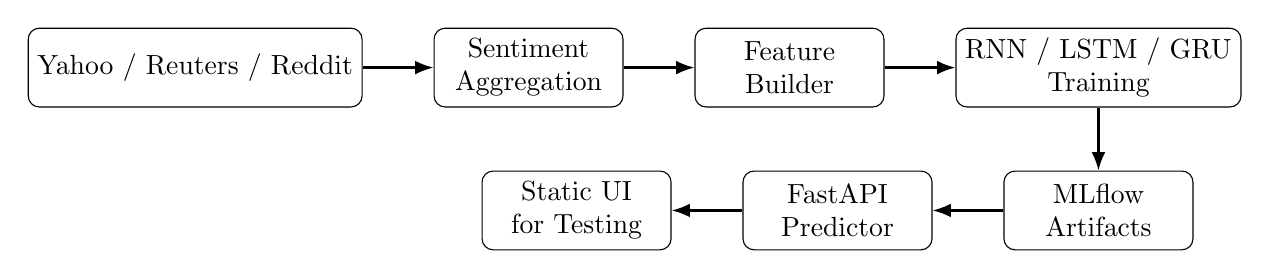
\begin{tikzpicture}[
  node distance=8mm and 9mm,
  block/.style={rectangle, draw, rounded corners, align=center, minimum width=24mm, minimum height=10mm},
  arrow/.style={-Latex, thick}
]
\node[block] (ingest) {Yahoo / Reuters / Reddit};
\node[block, right=of ingest] (sentiment) {Sentiment\\Aggregation};
\node[block, right=of sentiment] (features) {Feature\\Builder};
\node[block, right=of features] (train) {RNN / LSTM / GRU\\Training};
\node[block, below=of train] (mlflow) {MLflow\\Artifacts};
\node[block, left=of mlflow] (api) {FastAPI\\Predictor};
\node[block, left=of api] (ui) {Static UI\\for Testing};

\draw[arrow] (ingest) -- (sentiment);
\draw[arrow] (sentiment) -- (features);
\draw[arrow] (features) -- (train);
\draw[arrow] (train) -- (mlflow);
\draw[arrow] (mlflow) -- (api);
\draw[arrow] (api) -- (ui);
\end{tikzpicture}
\caption{High-level architecture of the market predictor pipeline.}
\end{figure}

\section{Data Collection}
The ingestion layer retrieves hourly OHLCV data from Yahoo Finance, business headlines from Reuters RSS, and social discussion from Reddit. Each source writes timestamped Parquet outputs, which allows the downstream stages to operate on recent snapshots without manual curation.

\section{Sentiment Analysis}
News and social text are classified with VADER for social posts and optionally FinBERT for Reuters headlines. The sentiment processor standardizes labels, extracts ticker symbols, and aggregates scores into hourly windows per ticker so that market and text data can be aligned on time.

\section{Time-Series Feature Construction}
The feature builder joins hourly sentiment with OHLCV data and constructs training windows. The resulting dataset includes returns, rolling volatility, and the core market features required by the sequential models. Table~\ref{tab:features} summarizes the feature groups used in the experiments.

\begin{table}[t]
\centering
\caption{Feature groups used in the time-series dataset.}
\label{tab:features}
\begin{tabular}{p{1.8cm}p{4.7cm}}
\toprule
Group & Examples \\
\midrule
Price & open, high, low, close, volume \\
Sentiment & net sentiment, mean score, text count \\
Derived & returns, rolling volatility, trend indicators \\
\bottomrule
\end{tabular}
\end{table}

\section{Modeling Approach}
The training script fits three sequential architectures: vanilla RNN, LSTM, and GRU. Each model learns to predict next-hour market direction from sliding windows of the aligned feature frame. Validation metrics are used for early stopping, and the best checkpoint is saved locally for serving.

\section{Experimental Setup}
The pipeline is configured to run locally, in Docker, or under Airflow. DVC manages the data lineage, MLflow records training parameters and test metrics, and GitHub Actions handles continuous integration plus deployment to EC2.

\section{Results}
Table~\ref{tab:results} will show the accuracy, F1 score, and comparative performance of the RNN, LSTM, and GRU models after final evaluation.

\begin{table}[t]
\centering
\caption{Placeholder for final model comparison results.}
\label{tab:results}
\begin{tabular}{lccc}
\toprule
Model & Accuracy & F1 & Notes \\
\midrule
RNN & 0.4830 & 0.0000 & Best checkpoint: models/rnn_best.pt \\
LSTM & 0.5166 & 0.6810 & Best checkpoint: models/lstm_best.pt \\
GRU & 0.5166 & 0.6803 & Best checkpoint: models/gru_best.pt \\
\bottomrule
\end{tabular}
\end{table}

\paragraph{Artifacts}
Final model checkpoints and MLflow artifacts are stored in the repository under `models/`, `mlruns/`, and `artifacts/` (see `artifacts/final_metrics.json` and `artifacts/collected_manifest.txt`).

\section{Deployment and MLOps}
The API exposes a prediction endpoint and a static frontend for manual testing. A Docker image packages the application, docker-compose supports local development, and the GitHub Actions workflow builds and deploys the image to EC2 using Docker Hub and SSH-based release automation.

\section{Conclusion}
This project demonstrates a reproducible MLOps pipeline for financial prediction that combines live data ingestion, sentiment analysis, sequential modeling, experiment tracking, and deployment. The remaining work is the final experimental sweep and reporting of the model comparison results.

\bibliographystyle{IEEEtran}
\begin{thebibliography}{00}
\bibitem{dvc} DVC, ``Data Version Control documentation,'' 2026.
\bibitem{mlflow} MLflow, ``Experiment tracking and model registry,'' 2026.
\bibitem{airflow} Apache Airflow, ``Workflow orchestration documentation,'' 2026.
\end{thebibliography}

\end{document}
